\documentclass[12pt,a4paper]{report}
\usepackage[czech]{babel}
\usepackage[T1]{fontenc}
\usepackage[utf8]{inputenc}

\usepackage{amsmath}
\usepackage{amssymb}
\usepackage{multirow}

\setlength\parindent{0.5cm}
\linespread{1.25}


%%% Údaje o práci
\def\NazevPrace{Vyčíslování chemických rovnic}
\def\AutorPrace{Václav Stupka}
\def\TridaAutora{8.M}
\def\SkolniRok{2021/2022}
\def\Seminar{Seminář z programování}
\def\DatumDokonceni{11. 2. 2022}

%% Definice různých užitečných maker (viz popis uvnitř souboru)
%%% Tento soubor obsahuje definice různých užitečných maker a prostředí %%%
%%% Další makra připisujte sem, ať nepřekáží v ostatních souborech.     %%%

%%% Užitečné balíčky (jsou součástí běžných distribucí LaTeXu)
\usepackage{graphicx}       % vkládání obrázků
\usepackage{indentfirst}    % zavede odsazení 1. odstavce kapitoly
\usepackage[nottoc]{tocbibind} % zajistí přidání seznamu literatury,obrázků a tabulek do obsahu
\let\openright=\clearpage
\usepackage{hyperref}
\hypersetup{unicode}
\hypersetup{breaklinks=true}

%%% Drobné úpravy stylu

% Tato makra přesvědčují mírně ošklivým trikem LaTeX, aby hlavičky kapitol
% sázel příčetněji a nevynechával nad nimi spoustu místa. Směle ignorujte.
\makeatletter
\def\@makechapterhead#1{
  {\parindent \z@ \raggedright \normalfont
   \Huge\bfseries \thechapter. #1
   \par\nobreak
   \vskip 20\p@
}}
\def\@makeschapterhead#1{
  {\parindent \z@ \raggedright \normalfont
   \Huge\bfseries #1
   \par\nobreak
   \vskip 20\p@
}}
\makeatother

% Toto makro definuje kapitolu, která není očíslovaná, ale je uvedena v obsahu.
\def\chapwithtoc#1{
\chapter*{#1}
\addcontentsline{toc}{chapter}{#1}
}

% Trochu volnější nastavení dělení slov, než je default.
\lefthyphenmin=2
\righthyphenmin=2




\newcommand{\s}{$ \rightarrow $}
\newcommand{\n}[1]{\mbox{#1}}
\newcommand{\sipka}{\rightarrow}

\begin{document}

%% Titulní strana a různé povinné informační strany
%%% Titulní strana práce a další povinné informační strany

%%% Titulní strana práce

\pagestyle{empty}
\hypersetup{pageanchor=false}

\begin{center}

{\large\textbf{Gymnázium Christiana Dopplera, Zborovská 45, Praha 5}}

\vspace{70mm}

{\Large ROČNÍKOVÁ PRÁCE}
\\ \vspace{4mm}
{\Huge\bfseries\NazevPrace}

\vfill
\end{center}

\begin{tabular}{ll}
Vypracoval: & \AutorPrace \\
Třída: & \TridaAutora \\
Školní rok: & \SkolniRok \\
Seminář: & \Seminar \\
\end{tabular}
\newpage

%%% Strana s čestným prohlášením k diplomové práci
\openright
\hypersetup{pageanchor=true}
\pagestyle{plain}
\pagenumbering{gobble}
\vglue 0pt plus 1fill

\noindent
Prohlašuji, že jsem svou ročníkovou práci napsal samostatně a výhradně s~použitím citovaných pramenů. Souhlasím s~využíváním práce na Gymnáziu Christiana Dopplera pro studijní účely.
\vspace{10mm}

\noindent V Praze dne \DatumDokonceni
\hfill
\AutorPrace

\vspace{20mm}
\newpage

\openright
\pagestyle{plain}
\pagenumbering{arabic}
\setcounter{page}{2}


%%% Strana s automaticky generovaným obsahem diplomové práce
\tableofcontents

\chapter{Úvod}
Tématem mojí ročníkové práce je naprogramovat aplikaci, která vyčísluje chemické rovnice. Spolu s tím je nutné navrhnout příslušný algoritmus. Tento dokument obsahuje tři kapitoly. V první z nich se zabývám obecnými informacemi o chemických rovnicích a základními principy jejich vyčíslování. Druhá kapitola je zaměřená na práci s maticemi při hledání řešení soustav lineárních rovnic -- na této metodě je založený algoritmus tohoto programu. Poslední kapitola slouží jako jednoduchá dokumentace vytvořené aplikace. Přílohy k dokumentu obsahují ukázku několika vzorových vstupů s příslušnými výstupy a také odkaz na GitHub, kde je volně k dispozici zdrojový kód mojí aplikace.

\chapter{Chemické rovnice}
Chemická rovnice se používá jako zápis chemických reakcí. Udává seznam látek, které se reakce účastní, a poměr jejich látkových množství (jinými slovy poměr počtu molekul jednotlivých sloučenin). Látky, které do rovnice vstupují, se nazývají reaktanty a zapisují se na levou stranu rovnice. Pravá strana vyjadřuje, které látky (tzv. produkty) danou reakcí vznikají. \cite{wiki}

\section{Zápis chemické rovnice}
Všechny reaktanty i produkty se zapisují svými chemickými vzorci. Před každou sloučeninou musí být uveden stechiometrický koeficient, tj. přirozené číslo vyjadřující relativní množství této látky vůči ostatním sloučeninám (číslo 1 se zpravidla vynechává). Obě strany rovnice se oddělují nejčastěji symbolem \s. Mezi jednotlivými reaktanty na levé a produkty na pravé straně rovnice se píše znaménko $ + $. \cite{wiki}

V případě, že v zápisu chemické reakce nejsou uvedeny stechiometrické koeficienty, nazývá se tento zápis reakčním schématem. Vyjadřuje pouze, které látky se reakce účastní, nikoli však jejich množství. Z toho důvodu se zpravidla nepoužívá. \cite{uch}

Příklady zápisu chemických rovnic:
\begin{align*}
 	2~\n{Na} + 2~\n{H}_2\n{O} &\sipka 2~\n{NaOH}+\n{H}_2\\
 	\n{CH}_4 + 2~\n{O}_2 &\sipka \n{CO}_2 + 2~\n{H}_2\n{O}\\
 	\n{P}_4\n{O}_{10} + 6~\n{H}_2\n{O} &\sipka 4~\n{H}_3\n{PO}_4
\end{align*}

Rovnice kromě toho může obsahovat i další údaje o vlastnostech chemických látek nebo průběhu reakce (např. skupenství látek, energie, další látky, které se účastní reakce, ale jejich množství se nemění -- tzv. katalyzátory). Tyto informace však nejsou podstatné pro potřeby této ročníkové práce. \cite{wiki}

\section{Vyčíslování chemických rovnic}
Proces, při kterém jsou do reakčního schématu doplňovány stechiometrické koeficienty, čímž vzniká chemická rovnice, se nazývá vyčíslování. Při něm se využívá několika chemických a fyzikálních zákonů, které musí každá chemická reakce splňovat.

Jedním z nich je zákon zachování hmotnosti. Z chemického pohledu je možné ho vyjádřit v následujícím znění: při reakci se zachovává počet a druh všech atomů. Pro chemickou rovnici to znamená, že celkový počet atomů jednoho prvku ve všech sloučeninách je stejný na obou stranách rovnice. Tento zákon je hlavní pomůckou při vyčíslování. \cite{uch}

Dále je možné použít také zákon zachování elektrického náboje, který říká, že celkový součet elektrických nábojů je stejný na obou stranách rovnice. Tím se zde ale nebudu zabývat, protože ho můj program nepoužívá.

\section{Postup při vyčíslování chemické rovnice}\label{postup_vycisleni}
Existuje několik metod, které lze při vyčíslování použít. Můj program používá postup založený výhradně na zákonu zachování hmotnosti.

Chemickou rovnici je možné převést na soustavu lineárních rovnic jejichž počet odpovídá počtu prvků ve sloučeninách. Neznámé této rovnice odpovídají ste\-chio\-metrickým koeficientům jednotlivých sloučenin. Způsobem, jak tuto soustavu vyřešit, se budu zabývat v následující kapitole. \ref{k2}

Protože se v těchto rovnicích nevyskytují absolutní členy (resp. jejich hodnota je vždy rovna 0), nebude mít tato soustava jednoznačné řešení. Jinými slovy pokud je řešením 
uspořádaná n-tice $ [a_1, a_2, \cdots, a_n] $, je řešením i $ [ka_1, ka_2, \cdots, ka_n], k \in \mathbb{N} $. To je možné dokázat pomocí substituce $ \forall i \leq n \wedge i \in \mathbb{N}: b_i = ka_i $. Po dosazení do soustavy a vynásobení všech rovnic číslem k získáme stejnou rovnici jako na počátku, ale místo kořenů $ a_i $ zaujímají kořeny $ b_i $, přičemž $ a_i \neq b_i $ Jako stechiometrické koeficienty se proto použije taková n-tice, jejíž členy jsou vzájemně nesoudělná přirozená čísla.


\subsection*{Příklad}
Při vyčíslení chemické rovnice $ \n{P}_4\n{O}_{10} + \n{H}_2\n{O} \sipka \n{H}_3\n{PO}_4 $ lze postupovat následovně:

Nejprve do rovnice doplníme neznámé na místo stechiometrických koeficientů:
$$ a~\n{P}_4\n{O}_{10} + b~\n{H}_2\n{O} \sipka c~\n{H}_3\n{PO}_4 $$

Chemickou rovnici je možné rozdělit na soustavu lineárních rovnic, jejichž počet odpovídá počtu prvků ve sloučeninách. Neznámými jsou potom stechio\-met\-ric\-ké koeficienty. V tomto případě bude soustava vypadat následovně:
\begin{align*}
	4a + 0b &= c&\mbox{(pro počty P)}\\
	10a + b &= 4c&\mbox{(pro počty O)}\\
	0a + 2b &= 3c&\mbox{(pro počty H)}
\end{align*}

Řešením je každá uspořádaná trojice $ [a, 6a, 4a], a\in \mathbb{N} $. Tato trojice je nesoudělná, pokud $ a = 1 $. Tudíž $ [a,b,c] = [1,6,4] $. Chemická rovnice tak má podobu:
$$ \n{P}_4\n{O}_{10} + 6~\n{H}_2\n{O} \sipka 4~\n{H}_3\n{PO}_4 $$

\section{Kontrola platnosti chemické rovnice}
Obecně je velice těžké posoudit, zda rovnice znázorňuje reálnou chemickou reakci. Přesto existuje jednoduchý způsob, jak některé rovnice snadno vyloučit. Jsou to ty, ve kterých není možné zajistit platnost zákona zachování hmoty. To se projeví tím, že stechiometrický koeficient alespoň jedné sloučeniny vyjde rovný 0.

Příklad:
$$a~\n{Na} + b~\n{H}_2\n{O} \sipka c~\n{NaOH}+d~\n{H}_2 + e~\n{Fe}$$
Soustava rovnic vypadá následovně:
\begin{align*}
	a &= c &\mbox{(pro prvek Na)}\\
	2b &= c + 2d &\mbox{(pro prvek H)}\\
	b &= c &\mbox{(pro prvek O)}\\
	0 &= e &\mbox{(pro prvek Fe)}
\end{align*} 
Nesoudělným řešením je $[a,b,c,d,e]=[2,2,2,1,0]$. Chemická rovnice má podobu:
$$2~\n{Na} + 2~\n{H}_2\n{O} \sipka 2~\n{NaOH}+1~\n{H}_2 + 0~\n{Fe}$$
Taková rovnice však nedává smysl. Můžeme ji proto vyloučit čistě na základě jejího vyčíslení. Jde o jedinou kontrolu, kterou můj program provádí.

\chapter{Řešení soustav lineárních rovnic pomocí matic}
\label{k2}
Jako postup pro řešení soustavy popsané v předchozí kapitole \ref{postup_vycisleni} jsem se rozhodl použít matici, kterou převedu pomocí elementárních úprav na specifický tvar, který je popsaný v další části této kapitoly. \ref{cilova_matice}

\section{Vyjádření chemické rovnice maticí \cite{czu}}
Mějme obecnou chemickou rovnici:
$$a_1~\n{A}_1 + a_2~\n{A}_2 + ... + a_m~\n{A}_m \sipka b_1~\n{B}_1 + b_2~\n{B}_2 + ...+ b_n~\n{B}_n,$$
kde $\n{A}_1, \n{A}_2, ..., \n{A}_m, \n{B}_1, \n{B}_2, ..., \n{B}_n$ jsou různé chemické sloučeniny. Lze ji převést na soustavu lineárních rovnic:
\begin{align*}
	c_{11}a_{1} + c_{12}a_{2} + \cdots + c_{1m}a_{m} &= d_{11}b_{1} + d_{12}b_{2} + \cdots + d_{1n}b_{n}\\
	c_{21}a_{1} + c_{22}a_{2} + \cdots + c_{2m}a_{m} &= d_{21}b_{1} + d_{22}b_{2} + \cdots + d_{2n}b_{n}\\
	c_{31}a_{1} + c_{32}a_{2} + \cdots + c_{3m}a_{m} &= d_{31}b_{1} + d_{32}b_{2} + \cdots + d_{3n}b_{n}\\
	&~...
\end{align*}
Koeficient $ c_{ij} $ vyjadřuje počet atomů $ i $-tého prvku ve sloučenině A$ _j $ a $ d_{ij} $ vyjadřuje počet atomů $ i $-tého prvku ve sloučenině B$ _j $.

Po převedení pravých stran rovnic na levé je možné k soustavě vytvořit její matici, která má podobu:
$$\mathbb{A} = \begin{pmatrix}
	c_{11} & c_{12} & \cdots & c_{1m} & -d_{11} & -d_{12} & \cdots & -d_{1n}\\
	c_{21} & c_{22} & \cdots & c_{2m} & -d_{21} & -d_{22} & \cdots & -d_{2n}\\
	c_{31} & c_{32} & \cdots & c_{3m} & -d_{31} & -d_{32} & \cdots & -d_{3n}\\
    \vdots & \vdots & \vdots & \vdots & \vdots  & \vdots  & \ddots & \vdots 
\end{pmatrix}$$
Rozšířená matice soustavy je potom:
$$\mathbb{A}|b = \begin{pmatrix}
	c_{11} & c_{12} & \cdots & c_{1m} & -d_{11} & -d_{12} & \cdots & -d_{1n} & \vline & 0\\
	c_{21} & c_{22} & \cdots & c_{2m} & -d_{21} & -d_{22} & \cdots & -d_{2n} & \vline & 0\\
	c_{31} & c_{32} & \cdots & c_{3m} & -d_{31} & -d_{32} & \cdots & -d_{3n} & \vline & 0\\
    \vdots & \vdots & \vdots & \vdots & \vdots  & \vdots  & \ddots &  \vdots & \vline & \vdots
\end{pmatrix}$$

Protože na pravé straně všech rovnic je 0, nebudu dále pravou stranu v~matici uvažovat, tj. pracovat budu pouze s maticí $ \mathbb{A} $.

\section{Zpracování matice}
Pro úpravu matice použiji všechny řádkové úpravy, tedy prohození dvou řádků, vynásobení řádku nenulovým číslem, přičtení jednoho řádku k jinému a vynechání nulového řádku. \cite{czu} Poslední jmenovanou úpravu zdroj nepovažuje za elementární, protože se při ní nezachovává velikost matice, pro účely této práce však bude vhodné ji taktéž použít.

\label{cilova_matice}
Cílem úprav je obdélníková matice. Počet jejích sloupců nadále odpovídá počtu sloučenin ($ m + n $) a v případě úspěchu je právě o jedna vyšší než počet řádků, který označím $ k = m + n - 1 $ (vzhledem k~odstraňování nulových řádků již nemusí odpovídat počtu prvků). Všechny prvky, které se nachází na \uv{diagonále} (tedy prvky $ a_{ii}, i \in N, i \leq k $), mají stejnou kladnou hodnotu, všechny prvky posledního, $(k+1) $-tého sloupce jsou záporné a všechny ostatní jsou rovny 0. Vypadá tedy následovně:
$$\mathbb{A} = \begin{pmatrix}
	p & 0 & 0 & 0 & \cdots & 0 & q_1 \\
	0 & p & 0 & 0 & \cdots & 0 & q_2 \\
	0 & 0 & p & 0 & \cdots & 0 & q_3 \\
    \vdots&\vdots&\vdots&\vdots&\ddots&\vdots&\vdots \\
	0 & 0 & 0 & 0 & \cdots & p & q_k \\
\end{pmatrix}$$
kde $ p \in \mathbb{N} $ a $q_1,q_2,q_3,\ldots,q_k \in \mathbb{Z}^- $. 

Aby všechny prvky matice zůstaly celočíselné, je nutné úpravy provádět podle určitých pravidel. Při přičítání řádků program vynásobí oba řádky tak, aby ve sloupci, ve kterém chceme nahradit prvek hodnotou 0, měly oba řádky opačnou hodnotu. Po každé úpravě je potřeba řádek vydělit nejmenším společným násobkem všech prvků tohoto řádku a nakonec ještě všechny řádky vynásobit tak, aby prvky \uv{diagonály} měly stejnou hodnotu.

\section{Získání stechiometrických koeficientů}
V případě, že se podaří matici upravit do tvaru popsaného v předchozí části, lze již tvrdit, že chemická rovnice bude vždy vyčíslitelná. Zároveň je také možné přímo získat nejjednodušší možný výsledek tvořený nesoudělnými stechiometrickými koeficienty:
\begin{align*}
	pa_1 &= q_1b_n\\
	pa_2 &= q_2b_n\\
	pa_2 &= q_3b_n\\
	     &\cdots \\
	pb_{n-1} &= q_kb_n
\end{align*}

Vzhledem ke způsobu, kterým jsem dospěl k těmto rovnicím, mohu tvrdit, že nejjednodušší řešení vypadá takto:
\begin{align*}
	a_1 &= q_1 \\
	a_2 &= q_2 \\
	&\cdots \\
	a_m &= q_m \\
	b_1 &= q_{m+1} \\
	b_1 &= q_{m+2} \\
	&\cdots \\
	b_{n-1} &= q_k \\
	b_n &= p
\end{align*}
Původní chemická rovnice má proto podobu:
$$q_1~\n{A}_1 + q_2~\n{A}_2 + ... + q_m~\n{A}_m \sipka q_{m+1}~\n{B}_1 + q_{m+2}~\n{B}_2 + ...+ p~\n{B}_n$$

Pokud matici do tohoto tvaru není možné upravit, mohou nastat dvě možnosti. Je-li počet sloupců roven počtu řádků, pak alespoň jeden z kořenů soustavy má nulovou hodnotu. Chemická rovnice je potom neplatná. Pokud je počet sloupců vyšší než počet řádků o více než jedna, pak by bylo nutné provést další kroky ke zjištění, zda existuje platné řešení a jakou má podobu. Můj program však tento postup neobsahuje a proto se jím nebudu zabývat.

\chapter{Ovládání programu}
Po spuštění aplikace se zobrazí okno, v jehož horní části se nachází menu. Zbytek okna tvoří textbox pro zadání chemické rovnice a tlačítko \uv{vyčíslit}, které spustí algoritmus vyčíslování. Finální, vyčíslená rovnice se zobrazí pod texboxem.

Kliknutím na pole \uv{nápověda} se zobrazí messagebox, který popisuje, jak má vypadat vstup zadaný do textboxu. Pole \uv{omezení} zobrazí messagebox informující o tom, které chemické rovnice program nedokáže zpracovat, ačkoli chemicky mohou být v pořádku. Pole \uv{vzorový vstup} vloží do texboxu ukázkovou chemickou rovnici a vyčíslí ji.

Vstup zadávaný do textboxu má podobu chemické rovnice bez stechiometrických koeficientů. Jednotlivé sloučeniny odděluje znaménko +, mezi stranami rovnice leží znaménko >. Na mezerách ve vstupu nezáleží, ale jedna sloučenina musí být zadaná bez mezer.

V případě nesprávného nebo neplatného vstupu mohou být vypsány tyto chybové hlášky:
\begin{description}
	\item[\uv{Rovnici se nepodařilo vyčíslit.}]~\\
	Vstupní chemickou rovnici program nedokázal vyčíslit, ačkoli to nemusí být nemožné.
	
	\item[\uv{Tuto rovnici nelze vyčíslit.}]~\\
	Zadanou chemickou rovnici není možné žádným způsobem vyčíslit.
	
	\item[\uv{Rovnice musí mít právě jedno znaménko >, které odděluje levou a pravou stranu.}]~\\
	Ve vstupu se nenachází žádné znaménko > nebo jich je naopak více než jedno.
	
	
	\item[\uv{Chybně zadaná sloučenina.}]~\\
	Ve vstupu se nachází např. dvě znaménka + za sebou nebo podobná chyba.
	
	\item[\uv{Počet atomů prvku ve sloučenině nemůže být číslo 0.}]~\\
	Alespoň jeden prvek se v některé sloučenině nachází v počtu 0 atomů.
	
	\item[\uv{Není možné vytvořit prázdnou závorku.}]~\\
	Ve vstupu se nachází levá a pravá závorka ihned za sebou, aniž by se v~ní vyskytovaly nějaké prvky.
	
	\item[\uv{Neplatný vstup.}]~\\
	Oznamuje jinou chybu vstupu, např. nepovolený znak.
	
	\item[\uv{Nastala neočekávaná chyba!!!}]~\\
	Oznamuje, že nastala chyba na úrovni frameworku .NET nebo v implementaci jazyka C\#.
\end{description} 
Program obsahuje i jiné chybové hlášky, které by se ale nikdy neměly vyskytnout.

\chapter{Závěr}
Vytvořil jsem program, jehož cílem je vyčíslovat chemické rovnice. Vysvětlil jsem, co to je a jakým způsobem ji lze vyčíslit. Základem aplikace je algoritmus pro řešení soustav lineárních matic, jehož popis je hlavní součástí této ročníkové práce. Jedná se o můj vlastní návrh, který je vhodný pouze pro tento účel -- pro obecné řešení soustav rovnic se nehodí. Na závěr jsem také ukázal, jakým způsobem se program používá a jakou podobu má mít vstup. Součástí této práce je také příloha s několika ukázkovými vstupy a příslušnými výstupy.

%%% Seznam použité literatury
\begin{thebibliography}{99}

\bibitem{uch}
Aleš Mareček, Jaroslav Honza. (1998): \textit{Chemie pro čtyřletá gymnázia.} Třetí opravené vydání. Olomouc: Nakladatelství Olomouc.\\
ISBN: 80-7182-055-5.

\bibitem{wiki}
Wikipedie. Chemická rovnice.\\
\url{https://cs.wikipedia.org/wiki/Chemick\%C3\%A1_rovnice}\\
(30. ledna 2022)

\bibitem{czu}
Soustavy lineárních rovnic\\
\url{http://dimatia.fav.zcu.cz/2005/vyuka/zm1/soustavy.pdf}\\
(30. ledna 2022)
\end{thebibliography}

%%% Prostor pro přílohy práce
\chapwithtoc{Příloha 1 - zdrojový kód}
Všechny zdrojové kódy mého programu, přeložený spustitelný soubor i tento dokument je k dispozici na adrese: \url{https://github.com/basvas-jkj/vycislovac_rovnic}.

\chapwithtoc{Příloha 2 - ukázka programu}
\begin{figure}[h]
	\centering
	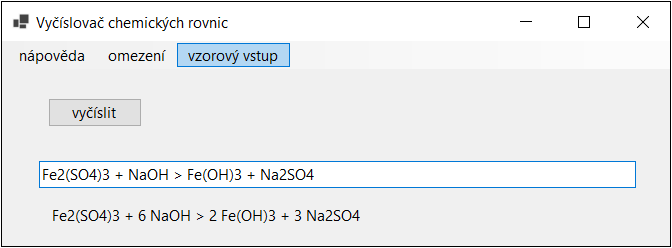
\includegraphics{vzorovy_vstup}
	\caption{vzorový vstup}
\end{figure}
\begin{figure}[h]
	\centering
	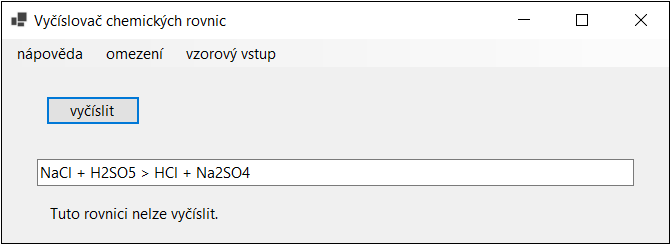
\includegraphics{nevycislitelna_rovnice}
	\caption{rovnice, kterou není možné vyčíslit}
\end{figure}
\begin{figure}[h]
	\centering
	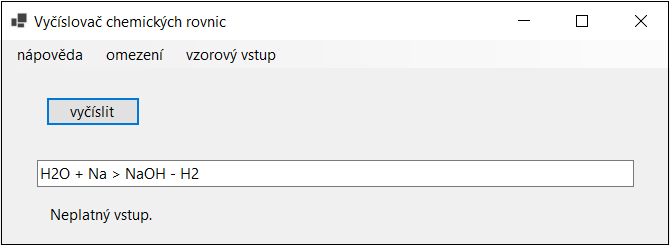
\includegraphics{chybny_vstup}
	\caption{ukázka chybného vstupu}
\end{figure}
\begin{figure}[h]
\centering
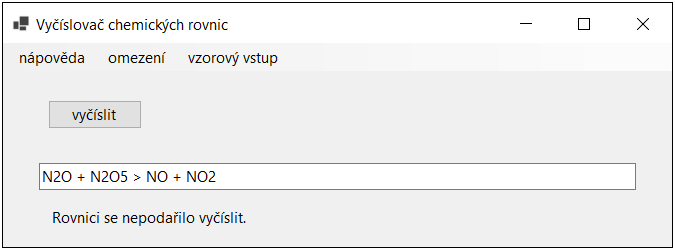
\includegraphics{nezvladnuta_rovnice}
\caption{rovnice, kterou program nedokázal vyčíslit, i když je to možné}
\end{figure}

\openright
\end{document}
